% Created 2018-11-29 Thu 18:38
\documentclass[presentation]{beamer}
\usepackage[utf8]{inputenc}
\usepackage[T1]{fontenc}
\usepackage{fixltx2e}
\usepackage{graphicx}
\usepackage{longtable}
\usepackage{float}
\usepackage{wrapfig}
\usepackage{rotating}
\usepackage[normalem]{ulem}
\usepackage{amsmath}
\usepackage{textcomp}
\usepackage{marvosym}
\usepackage{wasysym}
\usepackage{amssymb}
\usepackage{hyperref}
\tolerance=1000
\usepackage{xcolor}
\usepackage{listings}
\usetheme{default}
\author{Paul Bartholomew}
\date{\today}
\title{QuasIncompact3D 3D non-isothermal mixing layer}
\hypersetup{
  pdfkeywords={},
  pdfsubject={},
  pdfcreator={Emacs 24.5.1 (Org mode 8.2.10)}}
\begin{document}

\maketitle

\begin{frame}[label=sec-1]{QuasIncompact3D overview}
\begin{itemize}
\item Based on Incompact3D
\begin{itemize}
\item High-order compact finite-difference schemes
\item Highly scalable
\end{itemize}
\item Variable-density using Low Mach Number approximation
\begin{itemize}
\item Can solve pressure-Poisson approximately (fast)
\item Can solve pressure-Poisson exactly (slow)
\item Pseudo multiple fluids (free-surface implementation is current WIP)
\end{itemize}
\end{itemize}
\end{frame}

\begin{frame}[label=sec-2]{2D Validation: (Golanski et al. 2005)}
\begin{figure}[htb]
\centering
\includegraphics[width=0.75\linewidth]{./figures/golanski2d-rho.png}
\caption{Comparison of density contours at $t=24,82,182$ from top to bottom. Data obtained with QuasIncompact3D constant-coefficient Poisson solver, variable-coefficient Poisson solver ($\widetilde{\rho} = \rho_0, \rho^h$) and reference data (Golanski et al. 2005).}
\end{figure}
\end{frame}

\begin{frame}[label=sec-3]{2D Validation: (Golanski et al. 2005)}
\begin{figure}[htb]
\centering
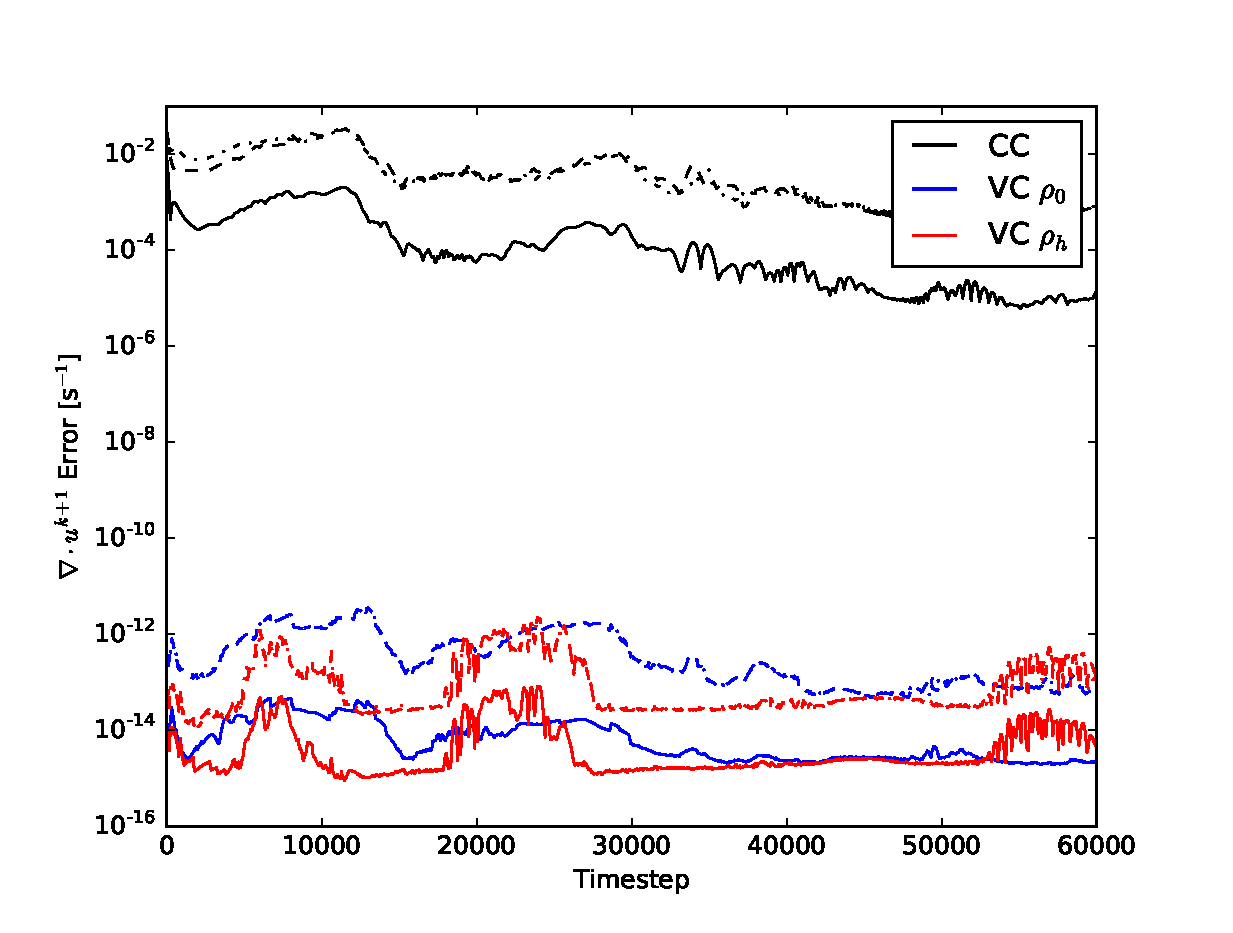
\includegraphics[width=0.75\linewidth]{./figures/err_divu.eps}
\caption{Comparison of errors in divergence constraint using QuasIncompact3D}
\end{figure}
\end{frame}

\begin{frame}[label=sec-4]{3D Mixing layer: setup}
\begin{figure}[htb]
\centering
\includegraphics[width=0.9\linewidth]{./figures/r1000-t0.png}
\caption{Initial velocity and density fields}
\end{figure}
\end{frame}

\begin{frame}[label=sec-5]{3D Mixing layer evolution}
\begin{figure}[htb]
\centering
\includegraphics[width=0.9\linewidth]{./figures/r2-t86-129-193-w03.png}
\caption{$\omega=0.3$ isosurface at $t=86,129,193$, $T_1 / T_2 = 2$, mesh: $64\times257\times64$}
\end{figure}
\end{frame}
% Emacs 24.5.1 (Org mode 8.2.10)
\end{document}